\subsubsection{Energetic Variational Inference Approach for Machine Learning}
Variational Inference (VI) is an important research area in the field of machine learning \cite{jordan1999introduction, blei2017variational}.
Its main idea is to convert the inference problem into an optimization problem, which aims at minimizing a certain functional that measures the difference between a distribution (whose pdf is denoted by $\rho$) and the target distribution (whose pdf is denoted by $\rho^*$) over a prescribed family of distributions $\mathcal{Q}$.
For example, using the Kullback--Leibler (KL) divergence, the VI problem is formulated as the following minimization problem.
\begin{equation}\label{eq:VI_KL}
\rho_{\text{opt}} =\text{arg}\min_{\rho \in \mathcal{Q} }\KL(\rho||\rho^*), \text{ where } \KL( \rho ||\rho^*)  = \int \rho(\x) \ln \left( \frac{\rho(\x)}{\rho^*(\x )} \right) \dd \x.
\end{equation}
There have been many VI approaches developed. 
They have a very broad application in machine learning.
Commonly, VI methods are used to approximate the posterior distribution for the Bayesian probabilistic models \cite{jordan1999introduction, neal1998view,  wainwright2008graphical, zhang2018advances}.
As alternatives to the MCMC sampling methods, VI methods are less computationally intensive and thus more suited to large datasets, and can be used whenever there is a need to explore many models \cite{blei2017variational}.
To highlight a few, there have been many works such as \cite{grave2011practical,welling2017multiplicative, wu2019deterministic,shridhar2019comprehensive} that combine the VI methods with Bayesian Neural Network.
The Gaussian process model is another popular supervised learning tool.
If it is combined with VI methods, its computational efficiency can be greatly improved as shown in \cite{king2006fast, nguyen2013efficient, nguyen2014automated, shetha2015sparse, damianou2016variational, cheng2017variational}.
The VI methods are also widely used in generative machine learning methods such as \cite{kingma2013auto, rezende2014stochastic, goodfellow2014generative,nowozin2016f, hu2017unifying} and in semi-supervised and unsupervised learning areas \cite{kingma2014semi,mnih2016variational,hu2017unifying}.
Broadly speaking, VI is a powerful tool for machine learning \cite{ma2019machine} and for the topics beyond the Bayesian statistics such as density estimation \cite{tabak2010density}.

In the recent work of Kang and her collaborators \cite{wang2021particle}, a new VI framework named \emph{energetic variational inference} or \emph{EVI} is introduced. 
It is a unified framework for the flow-based variational inference by employing the energetic variational approach \cite{liu2020variational},  which has been successfully used to study complicated systems in physics and biology.
Many new EVI methods can be obtained by using different choices of divergence functional \cite{amari2012differential} and dissipation laws \cite{liu2020variational}.
These new EVI methods can also be applied to machine learning problems, including Bayesian regressions, density estimations, and generative learning, etc. 
For example, the new version of the EVI method, called ``EVI-Im'' algorithm is compared with other competing algorithms on generating samples from a star-shaped mixture Gaussian distribution as shown in Figure \ref{fig:star}. 
The samples generated by EVI-Im has high fidelity to the target distribution and converges faster than the other algorithms. More details can be found in \cite{wang2021particle}. 
\begin{figure}[htbp]
\centering
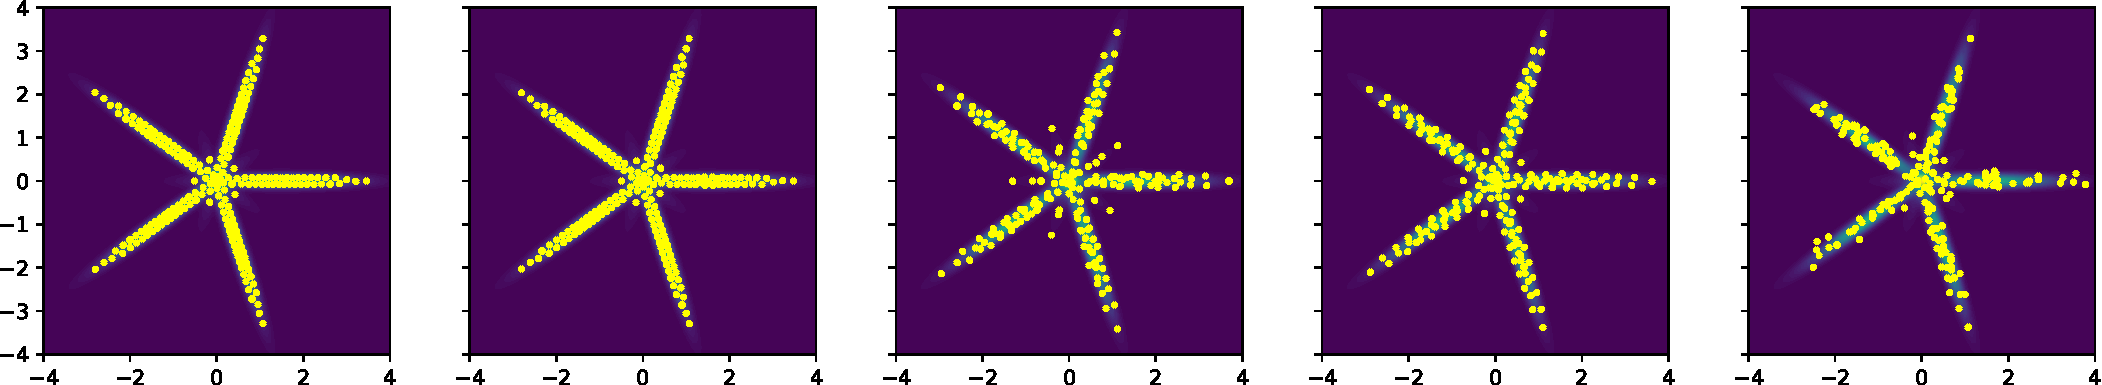
\includegraphics[width=\linewidth]{Star_compare}
\caption{ Particles obtained by various methods [200 particles]: (a) EVI-Im after 20 iterations, (b) Blob method (after 1000 iterations), (c) SVGD (after 1000 iterations), (d) matrix-valued SVGD (after 200 iterations) and (e) LMC (after 3000 iterations)}\label{fig:star}
%Particles obtained by various methods [200 particles]: EVI-Im after 20 iterations, Blob method and matrix-valued SVGD both after 1000 iterations; (b) cross-entropy v.s. number of iterations of the three methods.\label{fig:star}}
\end{figure}

SURE students will learn the foundations of variational methods and explore  and create new EVI algorithms by trying different combinations of divergence functionals and dissipation laws. 
They will develop new numerical schemes and build software based on them. 
SURE students will also explore new applications of the EVI algorithms in machine learning focusing on supervised learning models and generative learning models. 
They will work on interesting case studies with real-world data sets and problems. 
